\chapter{Datenverarbeitung und Vorverarbeitung }
\label{chap:vorverarbeitung}

In dieser Phase wurden die digitalisierten Rohdaten bereinigt und transformiert, um eine präzise Beantwortung der Forschungsfragen zu ermöglichen. Ein wesentlicher Bestandteil war die Überprüfung statistischer Voraussetzungen, um die Belastbarkeit der späteren Modelle sicherzustellen.

\section*{Datenbereinigung / Data Cleaning}
Bevor die eigentliche Analyse beginnen konnte, mussten die aggregierten Daten aus den verschiedenen Boroughs harmonisiert werden.
\begin{itemize}
    \item \textbf{Standardisierung:} Spaltenbezeichnungen wurden vereinheitlicht, um Inkonsistenzen zwischen den Teildatensätzen zu beseitigen. Dies umfasst z.b. die Korrektur von "Heads of Famlies" zu "Heads of Families".
    \item \textbf{Umgang mit Fehlwerten:} Da leere Felder in den historischen Tabellen oft das Nichtvorhandensein einer Gruppe signalisierten, wurden \textit{NaN}-Werte (Not-a-Number) durch Nullen ersetzt, um mathematische Berechnungen zu ermöglichen.
    \item \textbf{Deskriptive Vorstudie:} Es wurde eine deskriptive Statistik durchgeführt, um ein Gefühl für die Verteilungen und mögliche "Ausreißer-Berufe" zu erhalten.
\end{itemize}

Hieraus ließ sich folgender Boxplot für die Armutsraten erstellen:

\begin{figure}[htbp!]
    \centering
    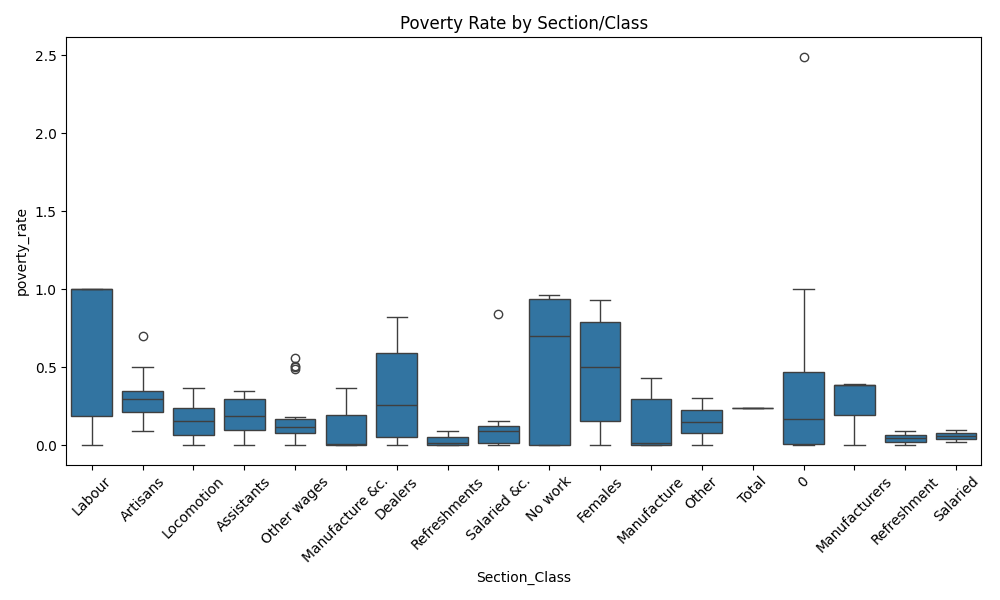
\includegraphics[width=1.2\textwidth]{contents/figures/boxplot_poverty_rate.png}
    \caption{Boxplot Armutsklassen}
    \label{fig:povertyClasses}
\end{figure}

\section*{Feature Engineering: Konstruktion von Metriken}
Um die Fragestellung nach Risikofaktoren operationalisierbar zu machen, wurden aus den Rohdaten neue Variablen berechnet:
\begin{itemize}
    \item \textbf{Poverty Rate:} Um die Armut messbar zu machen, wurde die Quote der Klassen A bis D im Verhältnis zur Gesamtbevölkerung einer Sektion berechnet: 
    \[ poverty\_rate = \frac{A + B + C + D}{Total} \]
    \item \textbf{Kids per Household:} Um die demografische Belastung zu erfassen, wurde die Anzahl der Kinder pro Haushaltsvorstand ermittelt (\textit{Children / Heads of Families}).
\end{itemize}

\section*{Statistische Voraussetzungsprüfung}
Ein zentraler Aspekt der Qualitätssicherung war die Überprüfung der Normalverteilung. 
\begin{itemize}
    \item \textbf{Shapiro-Wilk-Test:} Der Test auf die \textit{poverty\_rate} ergab eine Test-Statistik von 0,8229 und einen p-Wert von $9,11 \times 10^{-19}$.
    \item \textbf{Ergebnis:} Da der p-Wert weit unter der Schwelle von 0,05 liegt, wurde die Nullhypothese einer Normalverteilung abgelehnt. Die Stichprobe ist somit nicht-gaussisch (not Gaussian).
\end{itemize}

\section*{Methodische Konsequenzen}
Aufgrund der fehlenden Normalverteilung wurden die Analysepläne angepasst, um die Validität der Ergebnisse nicht zu gefährden:
\begin{itemize}
    \item \textbf{Nicht-parametrische Tests:} Für Gruppenvergleiche wurde der Kruskal-Wallis-Test anstelle einer ANOVA gewählt.
    \item \textbf{Korrelationen:} Die Zusammenhänge wurden mittels Spearman-Rangkorrelation anstelle von Pearson untersucht. Grund ist, dass die Spearman-Rangkorrelation robust gegenüber nicht-normalverteilten Daten ist.
    \item \textbf{Modell-Anpassung:} Für die Regression wurde ein transformiertes Modell (Log-Transformation) in Betracht gezogen, um die Residuen-Eigenschaften zu verbessern.
\end{itemize}

\begin{figure}[htbp!]
    \centering
    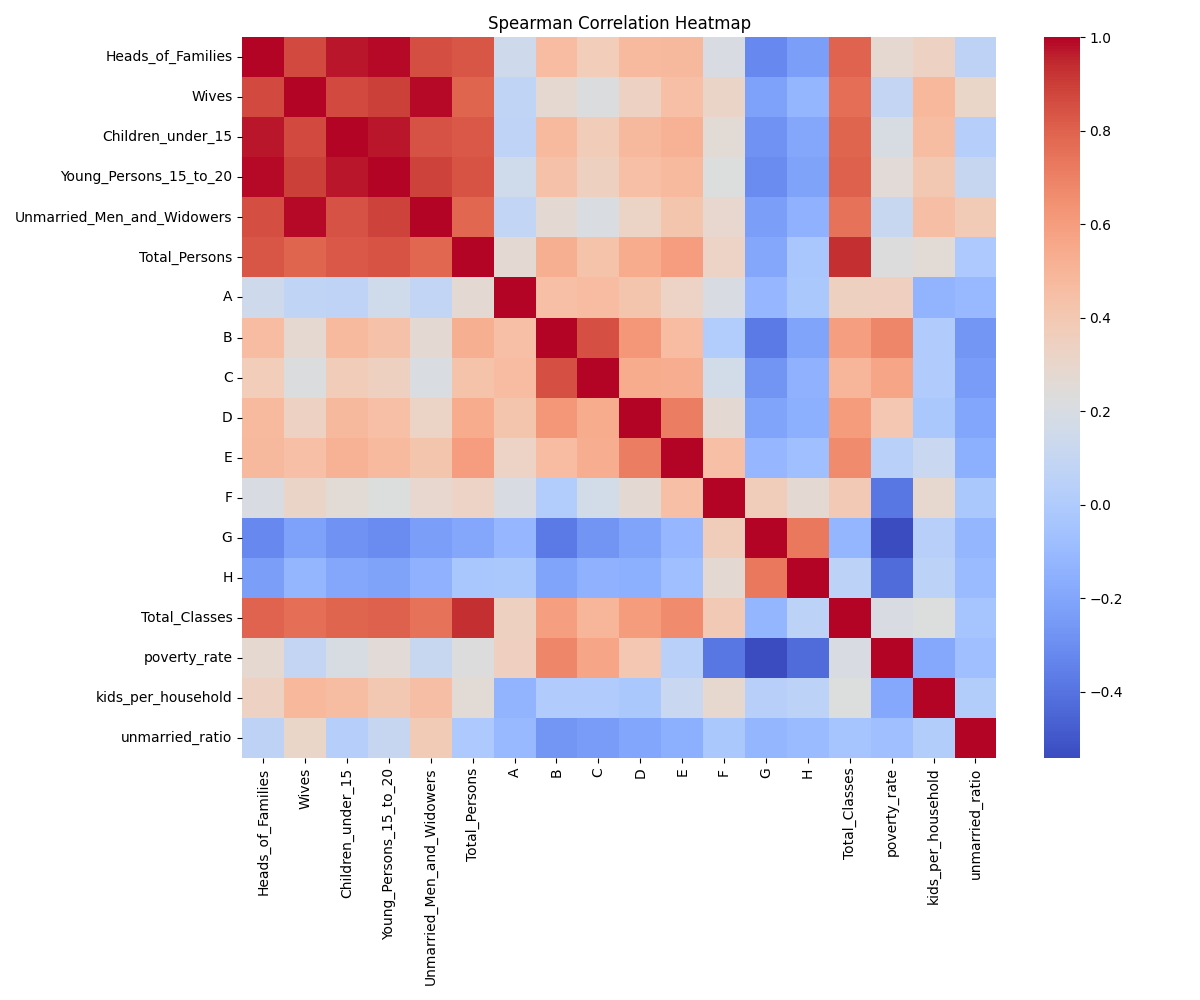
\includegraphics[width=0.85\textwidth]{contents/figures/correlation_heatmap.png}
    \caption{spearman correlation}
    \label{fig:spearman correlation}
\end{figure}